\documentclass[sigconf]{acmart}

%\usepackage{booktabs} % For formal tables
\usepackage{gensymb}
\usepackage{url}


% Copyright
%\setcopyright{none}
%\setcopyright{acmcopyright}
%\setcopyright{acmlicensed}
\setcopyright{rightsretained}
%\setcopyright{usgov}
%\setcopyright{usgovmixed}
%\setcopyright{cagov}
%\setcopyright{cagovmixed}


% DOI
\acmDOI{10.475/123_4}

% ISBN
\acmISBN{123-4567-24-567/08/06}

%Conference
\acmConference[WESE'18]{ACM Workshop on Embedded and Cyber-Physical Systems Education}{October 2018}{Turin, Italy}
\acmYear{2018}
\copyrightyear{2018}


\acmArticle{1}
\acmPrice{15.00}

% These commands are optional
%\acmBooktitle{Transactions of the ACM Woodstock conference}
%\editor{Jennifer B. Sartor}
%\editor{Theo D'Hondt}
%\editor{Wolfgang De Meuter}


\begin{document}
\title{Computers Interacting with the Physical World}
%\titlenote{Produces the permission block, and
 % copyright information}
\subtitle{A First-Year Course}


\author{Roger D. Chamberlain, Ron K. Cytron, Doug Shook, and Bill Siever}
%\author{Anonymous for review}
\affiliation{%
  \institution{Dept. of Computer Science and Engineering\\Washington University in St. Louis}
%  \institution{[Institution redacted]}
%  \streetaddress{One Brookings Dr.}
%  \city{Dublin}
%  \state{Ohio}
%  \postcode{43017-6221}
}
\email{{roger,cytron,dshook,bsiever}@wustl.edu}
%\email{[Email]}


% The default list of authors is too long for headers.
\renewcommand{\shortauthors}{R. D. Chamberlain et al.}
%\renewcommand{\shortauthors}{Anonymous for review}

%for comments
\newcommand{\FIXME}[1]{\textcolor{red}{FIXME: #1}}

\begin{abstract}
Abstract text goes here.
\end{abstract}

%
% The code below should be generated by the tool at
% http://dl.acm.org/ccs.cfm
% Please copy and paste the code instead of the example below.
%
 \begin{CCSXML}
<ccs2012>
<concept>
<concept_id>10010405.10010489</concept_id>
<concept_desc>Applied computing~Education</concept_desc>
<concept_significance>500</concept_significance>
</concept>
<concept>
<concept_id>10010520.10010553</concept_id>
<concept_desc>Computer systems organization~Embedded and cyber-physical systems</concept_desc>
<concept_significance>500</concept_significance>
</concept>
</ccs2012>
\end{CCSXML}

\ccsdesc[500]{Applied computing~Education}
\ccsdesc[500]{Computer systems organization~Embedded and cyber-physical systems}


\keywords{introductory course, cyber-physical systems}


\maketitle

\section{Introduction}
\label{sec:intro}

In the spring of 2015, the Dept.~of Computer Science and Engineering at
Washington University in St.~Louis decided to make a significant change
in its first-year course sequence for both computer science and
computer engineering majors.  While the first course follows, reasonably
closely, the CS1 curriculum from the ACM/IEEE~\cite{cs13}, our second semester
first-year course had a focus on thread-based parallelism.  The faculty
had collectively decided that the material in that course should be moved
to a later year (it is now offered as a sophomore-level technical elective),
and that a new course should be developed with a focus on how computers
interact with the physical world.
The new course was offered concurrently with the previous course in the
fall of 2015, and has been offered every semester since.
It is required for all computer science and computer engineering minors,
and is available as a technical elective to computer science minors (the
department does not offer a computer engineering minor) and electrical
engineering majors.

This paper describes that course: what we teach, how we teach it, and
what we have learned in the process.
The inspiration is that there is significant material that are core
computer science and computer engineering concepts which are well motivated
by the needs of computers as they interact with the physical world.
These include concepts such as information representation (e.g., digital inputs
and outputs represented at the bit level, analog input and output values as
non-negative binary integers with a given range),
timing (when something happens is a functional property of the program),
automata models (finite-state machines), etc.

The course is lecture-free, with students meeting twice a week in the
instructional laboratories.  One meeting per week is studio, in which the
students perform guided exercises aimed at the intellectual material we
expect them to master, and the other meeting is to work on assignments
that will be graded for assessment purposes.

The execution platforms used are built around the Arduino Uno~\cite{arduino},
which has an 8-bit AVR microcontroller as the processor,
and a traditional desktop (or laptop) machine that the
students program using Java (with the Eclipse IDE~\cite{eclipse}).
There are two specific advantages to using the Arduino platform.
First, it has a huge following in the maker/hobbyist community, which
is highly motivational for the students.  We regularly point them to
follow-on opportunities for extra-curricular projects.
Second, the simple 8-bit microcontroller at its core is conducive to
learning basic computer architecture and machine/assembly language
(which we include in the course as an additional core computer
science and engineering concept worthy of exposure in the first year).

There is an advantage to using Java with Eclipse as well. That is the
development environment the students use in the first semester course, so
it is familiar to them already as they enter.  This decreases the chance
of cognitive overload on purely logistical subjects, the Eclipse environment
is familiar, the Arduino development environment is very simple, the
Java language is familiar, and the Arduino C subset is quite close to
Java syntactically.

While there are a plethora of texts available within the Arduino
ecosystem, they are primarily targeting (and therefore better suited for)
the hobbyist community. Since
our course is intended to focus on core concepts, using the
Arduino platform for illustration and experimentation, we have authored
a text~\cite{cc17} for use with the course (which has the obvious
advantage of being well matched to the course goals).

The resulting course is well suited to the (admittedly differing) needs of
both computer science and computer
engineering students (e.g., we believe it is helping students discover
that they want to be computer engineers when they come into the course
not really knowing what computer engineering is).
In addition, we believe it is well positioned as an important course for
any student who wishes to be well educated in cyber-physical systems,
independent of major.
The subject matter is central to the National Academies' report on
cyber-physical systems education~\cite{nasem16}.

Unlike many introductory courses on embedded systems, which are upper-division
courses typically taken during the junior or senior year, this course is
designed to be a first-year course, accessible to students after only
one semester of introductory computer science.  With the proliferation of
computing well beyond the desktop and the server room, the sheer numbers
of computers that interact with the physical world are growing and
will continue to grow.
We believe that an early (first-year) introduction to the core concepts
introduced in this course is well deserved.

The organization of the paper is as follows.  Section~\ref{sec:topics}
articulates the intellectual material that we hope to impart on the
students.  
Section~\ref{sec:delivery} describes the educational approach used,
which is a member of the active learning family.
Section~\ref{sec:weeks} provides a brief syllabus, and
Section~\ref{sec:lessons} describes what we have learned as the course
was developed and taught over the course of seven semesters.
Section~\ref{sec:conclude} concludes and describes ideas we intend
to incorporate into future offerings of the course.

\section{Intellectual Topics}
\label{sec:topics}

While the course is aimed at first-year students, it is not intended to be a survey course.  It provides both exposure to and mastery of a variety of concepts in embedded and CPS, which are also significant components of the ACM's Computer Science and Computer Engineering curriculums~\cite{cs13,ce16}.  Below we describe what intellectual topics we cover in the course.  Items marked with an astrisk ($^*$)   indicate topics that students are expected to have significant mastery of while non-marked items indicate concepts with lesser depth.

\subsection{Information Representation}
\label{sec:ip}
\begin{itemize}
  \item Integer Representations: Both unsigned$^*$ and Twos compliment$^*$
  \item Hexadecimal and binary representations$^*$
  \item Non-Integer Numbers: Fixed point and IEEE-754 Floating Point
  \item Character Representations: ASCII$^*$ and Unicode
  \item Character strings, both as objects and as null-terminated C-style strings
  \item Use of fields in binary representations (as in Floating Point)
  \item Bitwise operations$^*$
  \item Arrays and memory organization
  \item Representation of real-world values as voltages that require conversion to a more appropriate unit (e.g., voltage to a temperature)$^*$
\end{itemize}

\subsection{Finite-State Machines}
\label{sec:fsm}
\begin{itemize}
\item Moore style finite state machines$^*$ are a fundamental component of multiple assignments.
\end{itemize}

\subsection{Timing and Events}
\label{sec:time}
\begin{itemize}
  \item Using delays in execution (or sleep) to control time-based behavior of devices$^*$
  \item Using delta timing techniques to maintain either a fixed period between actions or fixed rate of actions (assuming a feasible schedule)$^*$
  \item Using time-division multiplexing of a shared signal line
  \item The basic structure of an event loop for event-driven programming$^*$
\end{itemize}

\subsection{Physical I/O and Circuits Principles}
\label{sec:pio}
\begin{itemize}
  \item Physical buttons and the concept of ``bounce'' on real digital inputs$^*$
  \item Analog voltages and digitization of voltages (ADC)
  \item Pulse Width Modulation
  \item Ohm's Law and current constraints/current limiting$^*$
  \item Challenges of noisy data (e.g., step detection in accelerometer data)$^*$
\end{itemize}

\subsection{User I/O}
\label{sec:uio}
\FIXME{Should have a bullet/list}

\subsection{Communications}
\label{sec:comm}
\begin{itemize}
  \item Serial data exchanges$^*$
  \item Non-blocking communication$^*$
  \item Byte-ordering concerns when exchanging multi-byte entities$^*$
  \item Basic protocols and the exchange of tagged records$^*$
\end{itemize}

\subsection{Architecture / Assembly Language}
\label{sec:arch}
\begin{itemize}
  \item Assembly language for integer arithmatic$^*$
  \item Registers and register conventions$^*$
  \item Function call/use protocols$^*$
  \item Stack use conventions$^*$
  \item Memory organization$^*$
  \item C-style memory segmentation (Stack, Heap, and Text segments)
\end{itemize}

\section{Instructional Delivery and Materials}
\label{sec:delivery}

\subsection{Contact Time}

The class follows the \emph{flipped classroom} paradigm.  The course is lecture-free, with students meeting twice a week in the instructional laboratories.   One of the weekly meetings is an active learning \emph{studio session}.  The other meeting serves multiple needs: it's used for live-grading and in-person feedback on assignments, it's used as a convenient meeting time for group work, and it's also a time when all students should be able to meet with instructional staff for additional assistance with concepts or assignments.

For the last decade, the department has had a strong commitment to active learning~\cite{scbggg10,sgcggt10}. The evidence for the benefits of active learning is extensive~\cite{jjs98,lst99,Prince04,rss97}, and while actively learning is applied broadly, it is particularly compelling in science, math, and engineering design~\cite{Freeman14,lst99,Hake98,Byerley01,kb06}, including computer science~\cite{McConnell96,tlb01,skltc10,ag13}, computer engineering~\cite{hmdpa04,sr02}, and cyber-physical systems~\cite{me14,mmy16}.

Active learning is often associated with a flipped classroom.  In a flipped classroom contact time is spent \emph{actively} engaging with the course content, typically via applied problem solving or structured discussions. Whereas a significant amount of non-contact time is devoted to the content typically delivered via lecture, i.e., introducing conceptual material through either required readings or pre-recorded lecture videos.

A significant problem with the flipped classroom is that students make progress on posed problems at different rates. The approach we use across the entire first year is \emph{studio}-based~\cite{hnc08}. Our studio sessions evolved from observations by our colleagues in Art and Architecture who have a well established studio-based approach.  As elaborated below, elements present in these sessions include collaboration of 2-4 students with comparable work rates, continual feedback about product and process, and a problem to be solved by that group that lacks a unique answer or approach.  The sessions are guided but unscripted, with the students in a given group progressing at their own pace.

Collaboration like that used in the studio sessions may be particlarly well suited to attracting and retaining members of underrepresented groups. Studies~\cite{Krause:2012:EFL:2157136.2157192} have shown that women are attracted in greater numbers to computing when they appreciate the extent to which it is practiced collaboratively.  Moreover, because computing is largely collaborative, featuring collaboration early in the curriculum provides a more accurate representation to all students.  Consequently, studio sessions are intentionally collaborative and allow our students to enjoy learning by interacting with others and to develop group work skills.

Continual feedback during studio sessions is important to keep groups on task and to reinforce the importance of the material.  Feedback is given by the instructional staff, which include instructors as well as undergraduate Teaching Assistants (TAs). Courses are large (4 sections with 100+ students per section), but student-to-staff ratio is kept under 10 to 1 via a large number of TAs.  The bulk of TA work is logged during scheduled class sessions, where a TA is typically assigned to specific groups of students while instructors roam between the groups.  The use of primarily \emph{undergraduate} TAs may have some advantages.  Since many of the TAs have recently completed the same course, they have both recent exposure to the material and empathy for the challenges faced by their peers.  In addition, studies have shown that novices are more likely to predict the difficulty of a task for other novices than are experts~\cite{Hinds:1999}.

The studio groups are arranged by the students themselves, often determined by the way students seat themselves in the room. In our experience, a group functions best when its members are closest in ability, knowledge, and experience.  An opposite approach would form a team with some students who are capable enough to help the other students in the team.  We have found that resentment develops by all members in such situations, so we hope for teams with students at the same level.   We do not take steps directly to form such teams.  Instead, we encourage students to move between teams in the first few sessions, and they usually settle in a team that is comfortable for them.  Another important aspect of team work in studio is that we neither insist upon nor do we expect that teams should reach the end of all the work we assign in studio.  The idea is to plow deep, not far, and we grade students' studio sessions on participation, not on reaching any particular point in the studio work.  We encourage students to complete the studio work they did not finish in the 90-minute studio session outside our watch, on their own or with team members, as they prefer.

% TODO: Two thoughts about the above:  1) I'm not sure that we consistently encourage trying different groups (this should probably be stricter part of the instruction) and 2) Part of the above seems anicdotal --- can we provide supporting evidence?

Finally, the types of problems we pose in studio session are purposefully amenable to multiple solutions and approaches.  Examples from the first semester course include designing a flag and anthem for a fictitious country, determining how to draw a Sierpinski triangle, and throwing darts randomly at a dartboard to compute an approximation of $\pi$. Examples from this course include developing an algorothm to when a person has taken a step from accelerometer data and developing and implementing protocols to exchaning multiple types of messages between computers. Students know there is more than one way to solve any of these problems, which liberates them from finding the \emph{right} way and empowers them to find their \emph{own} way.  There are some potential downsides to this open ended structure.  First, in order to be able to provide assistance, instructional staff need to understand the unique approach being taken.  This, however, provides an opportunity for students in the course to practice communicating course content.   Second, some students are initially uneasy with the open-ended nature of the problems and are concerned about completing the task and finding the \emph{right} solution.  Providing cues that students should focus on process and understanding content rather than end product often helps alleviate these concerns.


\subsection{Tools and Platforms}

The execution platforms used are built around the Arduino Uno~\cite{arduino}, which has an 8-bit AVR microcontroller as the processor, and a traditional desktop (or laptop) machine programmed using Java (with the Eclipse IDE~\cite{eclipse}).

There are several advantages to using the Arduino platform.  First, it has a huge following in the maker/hobbyist community, which provides ample alternative sources of material and can motivate students to pursue extra-curricular projects.  Second, the simple 8-bit microcontroller at its core is conducive to learning basic computer architecture and machine/assembly language, Third, the Arduino IDE is crossplatform, so students can pursue work on their personal computers. Finally, although the platform is based on C++, a language unfamaliar to most students, the C++ conventions used by the platform make it easily accessible to students with Java experience, which was used in the prior course.

Java is also advantageous.  First, students in the course already have significant Java experience based on the prerequsite course.  Second, like Java is cross platform, again, students can work on their computers.  Finally, Java has a large set of libraries that leveraged as well as provide practice working with existing APIs.

While there are a plethora of texts available within the Arduino ecosystem, they  primarily target (and therefore better suited for) the hobbyist community.  Consequently, we have authored a text~\cite{cc17} for use with the course (which has the obvious advantage of being well matched to the course goals).

\subsection{Weekly Activities}

During a typical weekly module, students:
\begin{enumerate}
  \item prepare for studio sessions, by watching videos and/or completing required readings (prior to Monday),
  \item complete an on-line pre-studio quiz, which is intended to incentivize studio preparation but which only tests shallow knowledge from the module (prior to midnight Sunday),
  \item participate in the studio session (class Monday),
  \item complete and do a live demo of an assignment from the previous module (class Wednesday),  and
  \item complete an on-line summary quiz of the previous module (by midnight Wednesday). Summary quiz questions are more subtantial than pre-studio quizzes and are often comparable to exam questions.
\end{enumerate}


\subsection{Student Assessment}

The assessment of students takes a number of forms, including studio participation (15\%), on-line quizzes (15\%), assignments (35\%), and three exams (10\% each).
% TODO: BSIEVER: Check the above numbers

Due to the open-ended nature of studio sessions and the desire to emphasize process and understanding, studio sessions are graded based on  participation.

Assignments are graded based on a rubric.  Students are provided with a summary of the major points in the rubric, but details such as specific testing procedures are often not provided.  The rubrics often evaluate functionality of a submission (does it work?) as well as design decisions (did they choose an appropriate approach?) and implementation details (coding style, etc.). Our TAs are then provided with a rubric that may include finer granularity (i.e., specific points based on appropriate code indentation) or specific testing procedures. Students must show their work to a TA who will complete the rubric and submit the grade for that assignment.

At three points during the semester (approximately evenly spaced) there is a written exam.  During each of those weeks, the studio session is tailored to have review content, the second laboratory meeting during the week does not have an assignment due, and the
exam is scheduled at a common time for all studnets.  In some semesters, the last exam has been comprehensive, but currently it merely covers the last third of the material.

\section{Modules}
\label{sec:weeks}

\FIXME{Module descriptions.}

\paragraph{Information Representation} Implementing finite-state machines.
Bit-manipulation operations.

\paragraph{Microcontroller Platform} Designing finite-state machines.
Digital input and output.

\paragraph{Real-Time Computing} Analog input. Simple filtering.

\paragraph{Computer Communications - 2 weeks} Protocol design.

\paragraph{Multiplexing} Pixel-based displays.

\paragraph{Integrative Project} Acceleration. Pedometer. Predator-prey game.

\paragraph{Computer Architecture and Assembly Language - 3 weeks} Data layout.
Program control. Arrays in memory.

\FIXME{Available modules not in current use.}

\paragraph{Interrupts}

\paragraph{IP Networking}

\section{Lessons Learned%
\protect\footnote{The work is under the oversight of the IRB at Washington Univ. in St. Louis.}
}
\label{sec:lessons}

%Next, we describe the lessons we have learned over the span of several
%offerings of the course

\subsection{Pacing of Material}

%\FIXME{Assignments with a duration of only one week.}

As recently as the spring semester of 2017, the pacing of material
was uneven and somewhat too fast.  The following are quotes from
end-of-semester student evaluations.
\begin{itemize}
\item ``The pace was inconsistent.''
\item ``It moved a little too fast in parts and wasn't always as
in-depth as I would've liked.''
\item ``We moved pretty quickly through material and I never felt like I had
time to fully grasp concepts because the assignments took so much time.''
%\item ``The class moved too quickly.''
%\item ``Assignments were too long for such short period of time.''
\end{itemize}
In reaction to these comments, we've evolved the course into the organization
that is described in Section~\ref{sec:weeks}.
For example, the networking module was (at least temporarily) retired
and the assembly language material was converted from a
2 week series into a 3 week series, without expanding the content.

The results of the pace ratings for spring 2018 are shown in
Figure~\ref{fig:pace} (using a 7-item Likert scale).
The mean score of 5.47 (std. dev. of 1.41)
is very close to the department's average of
5.66, and a substantial improvement from the mean score of 4.51
for the course in spring of 2017.

\begin{figure}[t]
\centering
\parbox{0.48\columnwidth}{%
   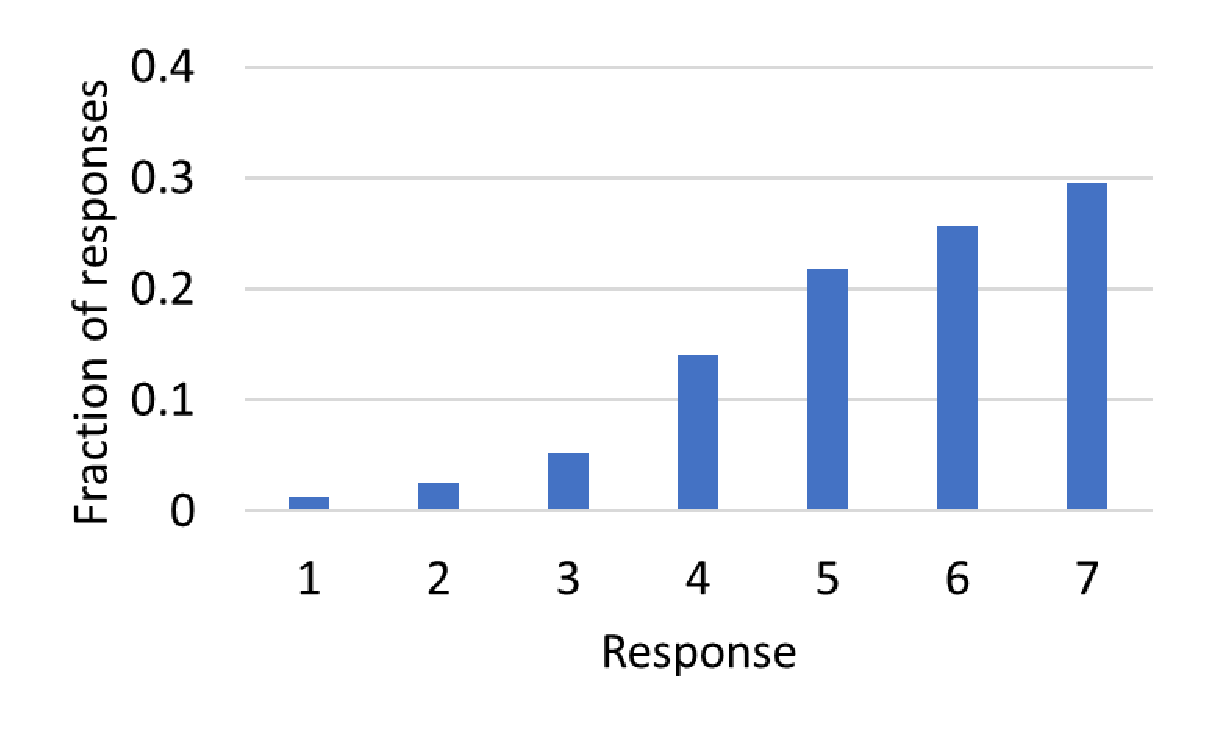
\includegraphics[width=0.47\columnwidth]{pace}
   \caption{Student ratings of statement, ``The material was covered
at a reasonable pace''  (scoring: 1 - Strongly Disagree, 7 - Strongly Agree).}
   \label{fig:pace}
}
~
\parbox{0.48\columnwidth}{%
   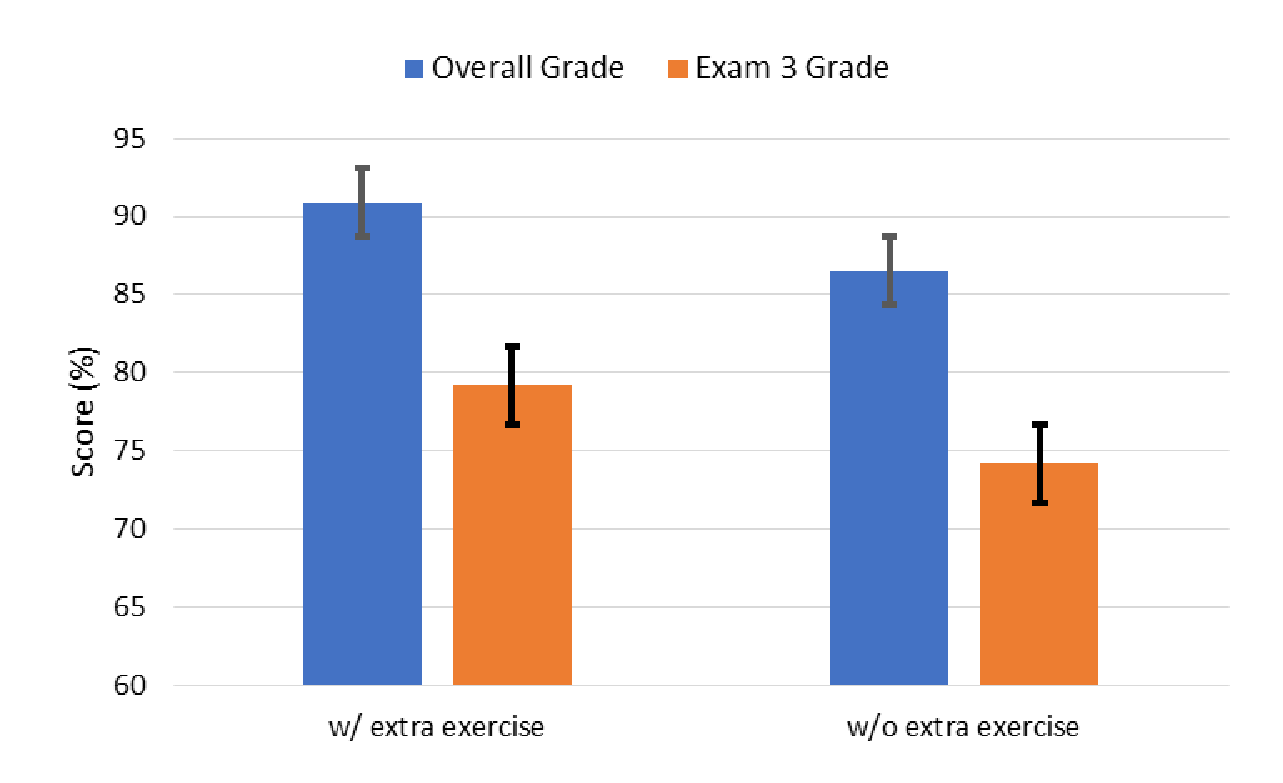
\includegraphics[width=0.47\columnwidth]{scores}
   \caption{Relationship between overall scores and exam~3 scores
with and without the extra exercise. Bars indicate mean and
whiskers std.~err.}
   \label{fig:scores}
}
\end{figure}

\subsection{Analysis Problems}

Based on commentary in the literature that posits the benefits of
analysis problems in the context of design courses~\cite{wjbo01},
we were concerned that the present
course doesn't have sufficient analysis content (i.e., the bulk of
studio questions and assignment questions are design questions rather
than analysis questions).

To test this theory, we generated an additional set of analysis problems,
designed to be helpful in preparing students for the third exam, and
made them available to students one week prior to the exam.  To provide
an incentive for the students to attempt them, students were told that
there would be a small amount of extra credit for those that did well.

We then compared scores for the two groups of students, those who did
attempt the extra credit exercise and those who did not.  The results
of this comparison are shown in Figure~\ref{fig:scores}.
There clearly is a correlation between overall course grade and
whether or not a student attempted the extra exercise.
Those who attempted the extra exercise scored over 4\% higher overall
(the scores presented exclude the extra credit provided from the
exercise).  This is statistically significant ($p = 0.02$, non-paired data).
When we examine the scores on exam~3, however, the story is different.
While the mean score differential is similar (at 5\% in this case), the
variability in scores is wide enough that this result is not
statistically significant ($p = 0.11$, non-paired data), so we cannot
rule out the null hypothesis that the difference in the means is
due to chance.

Our current opinion is that the correlation seen in the overall scores
is likely due to the
fact that better students (more likely to achieve a higher score prior
to the availability of an optional exercise) are also more likely than
their peers to take advantage of an optional exercise, especially when
it provides extra credit.
Going forward, we are still interested in whether or not additional
analysis problems can help students learn the material better, and will
likely pursue it by altering the mix of analysis vs.~design problems
within the studio exercises.

\subsection{Logistics}

%In general, the logistics of the course haven't been as smooth as they could be.
%A couple quotes from recent student evaluations (spring 2018):
%\begin{itemize}
%\item ``More structure and organization, use more difficult examples when
%teaching the material since the assignments were a lot harder than
%the given examples.''
%\item ``It needs more organization.''
%\end{itemize}
%This past semester we didn't do as good a job as we should have
%in communicating due dates, etc. A number of the specifics on the calendar
%were filled out (made available to the students) as the semester proceeded.
%In retrospect, this was a mistake, as a number of things didn't make it on
%to the calendar early enough for everyone to see them.

The removal of a live lecture session in favor of on-line videos has been
a challenge for some students. Since videos are static content, there is an
extra layer of effort that students must take if they do not understand the
presented concepts or need additional explanation. Interactions with professors
are also fewer and farther between as students are spread out across multiple
computer labs instead of meeting as a single, large group.

In the fall of 2017, we introduced a recitation section to address these issues.
The recitation sections would occur after the weekly studio, but before the weekly
assignment was due, so students could ask questions about topics they had
seen in the on-line videos and studio. The effect of these recitation sessions
was somewhat mixed, as shown by comments on student evaluations:
\begin{itemize}
\item ``I only attended a handful of the recitation, specifically when I was
confused on a topic, and every time I came my questions were answered and
it was very helpful."
\item ``Kind of a waste of time."
\end{itemize}

A common complaint is that recitation sessions were short and
unstructured. While they were intended to be loosely
structured and student-driven by design, a more structured approach with
pre-prepared review questions and practice problems may prove to be
more beneficial for students.

%Like many computer science programs, we are seeing an increase in
%the number of students enrolled in our courses. This led to a bottleneck
%during assignment submission time, as having students demo their work
%took time and there would also inevitably be a number of students who had
%last minute problems that needed to be solved before they could submit their
%assignment. This combination was putting a strain on our TAs, and students
%were having difficulty getting the help that they needed on these busy days.

%This past semester, the professors of the course started holding office hours in
%one of the nearby computer labs during these busy times. Students who had
%problems with that week's assignment had a direct line to someone who could
%help them, which freed up the TAs to focus on demoing completed assignments.
%This setup greatly increased the efficiency of assignment submissions and will
%likely be continued in future semesters.

\section{Conclusions}
\label{sec:conclude}

We have described a first-year course that we feel is appropriate
for both computer science and computer engineering majors. For example,
we believe it is helping students discover
that they want to be computer engineers when they come into the course
not really knowing what computer engineering is.

With the proliferation of
computing well beyond the desktop and the server room, the sheer numbers
of computers that interact with the physical world are growing and
will continue to grow.
We believe that an early introduction to the core concepts
introduced in this course is well deserved.


\section*{Acknowledgements}
The authors would like to acknowledge
the generous support of the Larsen family, which has been instrumental
in the development of this course.

\bibliographystyle{ACM-Reference-Format}
\bibliography{paper}

\end{document}
